\documentclass{mini}
\usepackage[utf8]{inputenc}
\usepackage{caption}
\usepackage{subcaption}
\usepackage[polish]{babel}
\usepackage{graphicx}
\usepackage{mathtools}
\usepackage{algpseudocode}
\usepackage{color}
\usepackage{xcolor}
\usepackage{listings}
\usepackage{catchfilebetweentags}
\usepackage{enumitem}

\usepackage{catchfilebetweentags}
\usepackage{etoolbox}
\setcounter{tocdepth}{2}
\makeatletter
\patchcmd{\CatchFBT@Fin@l}{\endlinechar\m@ne}{}
  {}{\typeout{Unsuccessful patch!}}
\makeatother

\addto\extraspolish{%  
 \def\figureautorefname{Rysunek}%  
} 

%------------------------------------------------------------------------------%
\title{Realizacje scenariuszy działań}
\pm{Robert Jakubowski}
\author{Mariusz Ambroziak
\\Paweł Bielicki
\\Karol Bocian
\\Hanna Dziegciar
\\Karol Dzitkowski
\\Mateusz Jankowski
\\Wiktor Ryciuk}
\monthyear{\today}
%------------------------------------------------------------------------------%
\begin{document}
%<*tag>
\section{Przykłady}

\subsection{Pytanie czy dany scenariusz moze wystąpić}

\subsubsection{Historia}

Michał jest pracującym  studentem. W środę powinien o godzinie 8.00 pojawić się w pracy zupełnie trzeźwy, a mimo to we wtorek postanowił pójść do baru. Jeśli Michał się napije,  stanie się pijany. Jeśli pójdzie spać przestanie być pijany, ale stanie się skacowany, co również będzie niedopuszczalne w w jego pracy.

\subsubsection{Opis akcji}

 \textbf{initially}  \textit{$\neg$drunk \textbf{and} $\neg$hangover}\\
 \textit{(drink,2)}  \textbf{ causes}  \textit{drunk}\\
\textit{(sleep,8)}   \textbf{causes} \textit{$\neg$drunk}\\
\textit{(sleep,8)}   \textbf{causes} \textit{hangover}  \textbf{if}  \textit{drunk}\\


\subsubsection{Scenariusze}

Sc =$(OBS,ACS)$\\
OBS =  $ {\{(\neg drunk,10), (\neg hangover,10)\} }$\\
ACS = ${\{((drink,2),0),((sleep,8),2)\}}$\\


Sc2 =$(OBS2,ACS2)$\\
OBS =  $ {\{(\neg drunk,10), (\neg hangover,10)\} }$\\
ACS = ${\{((sleep,8),1)\}}$\\


\subsubsection{Kwerendy}

\begin{enumerate}
	\item  \textbf{ever executable} \textit{Sc}
	\item  \textbf{ever executable} \textit{Sc2}
\end{enumerate}

\subsubsection{Analiza}

Odpowiedzi na kwerendy to odpowiednio:
\begin{enumerate}
	\item \texttt{FALSE},
	\item \texttt{TRUE},
\end{enumerate}

Zgodnie z diagramem dla scenariusza  \textit{Sc}

\begin{center}
  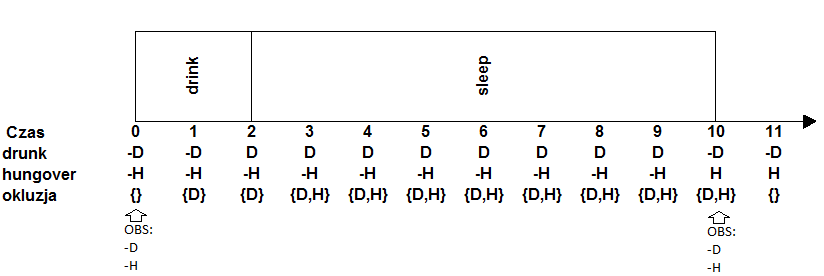
\includegraphics[width=1\textwidth]{Example1}
\end{center}

Zgodnie z diagramem dla scenariusza  \textit{Sc2}

\begin{center}
  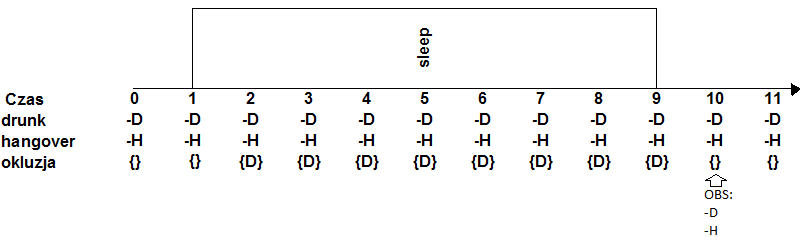
\includegraphics[width=1\textwidth]{Example1a}
\end{center}

Scenariusz \textit{ Sc2} jest w pełni poprawny i wykonywalny. Scenariusza \textit{Sc} nie można wykonać, ponieważ wymaga on by w chwili 10 fluenty \textit{drunk} i \textit{hangover} miały wartość FALSE, jednak w tej chwili zmienna \textit{hangover} ma wartość TRUE.


\subsection{Pytanie czy dany warunek zachodzi w danym czasie}

\subsubsection{Historia}

Mick i Sarah są parą, więc mają wspólne produkty spożywcze, ale posiłki zwykle jadają oddzielnie. Pewnego dnia Sarah chce zrobić ciasto, a Mick naleśniki. Nie mogą być one robione w tym samym czasie ze względu konieczność użycia miksera do przygotowania obu. Ponadto, zrobienie jednego lub drugiego dania zużywa cały zapas jajek dostępnych w mieszkaniu, więc trzeba je potem dokupić.

\subsubsection{Opis akcji}
 \textbf{initially}  \textit{eggs}\\
$(making\_panc,1)$   \textbf{causes} $\neg$\textit{eggs} \textbf{ if } \textit{eggs}\\
$(making\_cake,1)$   \textbf{causes} $\neg$\textit{eggs} \textbf{ if } \textit{eggs}\\
$(buy\_eggs,2)$  \textbf{causes}  \textit{eggs}\\


\subsubsection{Scenariusz}

 \textit{Sc} =$(OBS,ACS)$\\
 \textit{OBS} =  ${\emptyset}$\\
 \textit{ACS} = $\{((making\_panc,1),0), ((making\_cake,1),2)\}$


\subsubsection{Kwerendy}

\begin{enumerate}
	\item  \textit{eggs}  \texttt{at} 0  \textbf{when}  \textit{Sc}
	\item  \textit{eggs} \texttt{at} 2 \textbf{ when} \textit{ Sc}
\end{enumerate}

\subsubsection{Analiza}

Odpowiedzi na kwerendy to odpowiednio:
\begin{enumerate}
	\item \texttt{TRUE},
	\item \texttt{FALSE}.
\end{enumerate}
	
	Zgodnie z diagramem dla scenariusza \textit{Sc}:

\begin{center}
  
\includegraphics[width=1\textwidth]{Example2}
\end{center}

	Oczywiście warunek akcji \textit{making\_panc} nie jest spełniony w momencie $2$.

\subsection{Pytanie czy dana akcja jest wykonywana w pewnym czasie}

Ten przykład pokazuje przypadek kwerendy, która pyta, czy dana akcja jest wykonywana w pewnym czasie.

\subsubsection{Historia}

Mamy Billa i psa Maxa. Jeśli Bill idzie, to Max biegnie przez jakiś czas. Jeśli Bill gwiżdże, Max szczeka przez jakiś czas. Jeśli Bill zatrzymuje się, Max również. Jeśli Bill przestaje gwizdać, to Max przestaje szczekać.

\subsubsection{Opis akcji}

\textbf{initially} $\neg run\_Max$ \textbf{and} $\neg bark\_Max$ \\
$(goes\_Bill,2)$ \textbf{causes} $run\_Max$\\
$(goes\_Bill,2)$ \textbf{invokes} $(runs\_Max,2)$ \textbf{after} $0$\\
$(runs\_Max,2)$ \textbf{causes} $\neg run\_Max$\\
$(whistles\_Bill,1)$ \textbf{causes} $bark\_Max$\\
$(whistles\_Bill,1)$ \textbf{invokes} $(barks\_Max,1)$ \textbf{after} $0$\\
$(barks\_Max,1)$ \textbf{causes} $\neg bark\_Max$\\


\subsubsection{Scenariusz}

\textit{Sc} =$(OBS,ACS)$\\
\textit{OBS} = ${\emptyset}$\\
\textit{ACS} = $\{ ((goes\_Bill,2),1), ((whistles\_Bill,1),5),((goes\_Bill,2),7)\}$\\

\subsubsection{Kwerendy}

\begin{enumerate}
\item \textbf{performing} $runs\_Max$ \textbf{at} $8$ \textbf{when} \textit{Sc}
\item \textbf{performing} $runs\_Max$ \textbf{when} \textit{Sc}
\item \textbf{performing} \textbf{at} $8$ \textbf{when} \textit{Sc}
\end{enumerate}

\subsubsection{Analiza}
Odpowiedzi na powyższe kwerendy są następujące:
\begin{enumerate}
\item \texttt{FALSE},
\item \texttt{TRUE},
\item \texttt{TRUE}.
\end{enumerate}
Ilustruje to poniższy diagram:

\begin{center}
  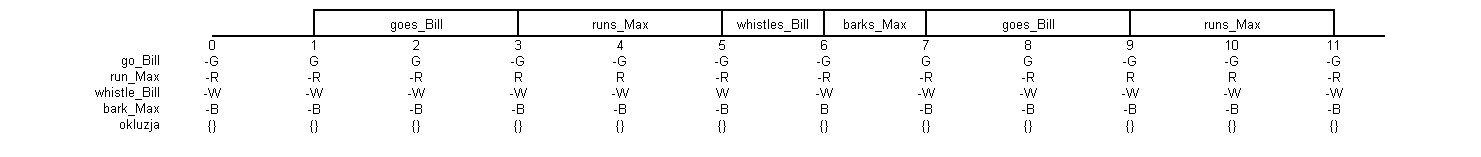
\includegraphics[width=1\textwidth]{Example3}
\end{center}

\subsection{Brak integralności}

Przykład \textit{Brak integralności} pokazuje scenariusz, który mimo zgodności z warunkami zadania, jest sprzeczny z logiką \textit{common sense} (z powodu braku warunków integralności).

\subsubsection{Historia}
Mamy Billa oraz komputer. Bill może nacisnąć przycisk \textit{Włącz} lub odłączyć komputer od zasilania. Komputer jest wyłączony i podłączony do zasilania. Jeżeli zostanie naciśnięty jego przycisk \textit{Włącz}, to komputer włączy się. Odłączenie komputera od prądu powoduje, że komputer  będzie odłączony od zasilania.

\subsubsection{Opis akcji}

\textbf{initially} $\neg on\_computer$ \textbf{and} $connect\_power\_computer$\\ 
$(clicks\_button\_on,1)$ \textbf{invokes} $(switches\_on\_computer,2)$ \textbf{after} $0$\\
$(switches\_on\_computer,2)$ \textbf{causes} $on\_computer$\\
$(disconnects\_power,1)$ \textbf{causes} $\neg connect\_power\_computer$

\subsubsection{Scenariusz}

\textit{Sc} =$(OBS,ACS)$\\
\textit{OBS} = ${\emptyset}$\\
\textit{ACS} = $\{(clicks\_button\_on,1),1),((disconnects\_power,1),4),((clicks\_button\_on,1),5)\}	$\\

\subsubsection{Kwerendy}

\begin{enumerate}
\item $on\_computer$ \textbf{at} $8$ \textbf{when} \textit{Sc}
\end{enumerate}
Znak zapytania oznacza, że stan w tym przypadku nie zgadza się ze zdrowym rozsądkiem.


\subsubsection{Analiza}
Powyższy scenariusz jest prawidłowy, lecz zawiera pewną niezgodność. W chwili $t = 4+1$ komputer zostaje odcięty od zasilania. Powinien więc wyłączyć się. Bill w chwili $t = 5+1$ naciska przycisk \textit{Włącz}. Komputer zacznie włączać się mimo iż jest odcięty od zasilania. Zachodzą dwa sprzeczne ze sobą z  punktu widzenia zdrowego rozsądku  stany, tj. $connect\_power\_computer=\neg C $  i $on\_computer=N$. Odpowiedzi na powyższą kwerendę będzie \texttt{TRUE}.

\begin{center}
  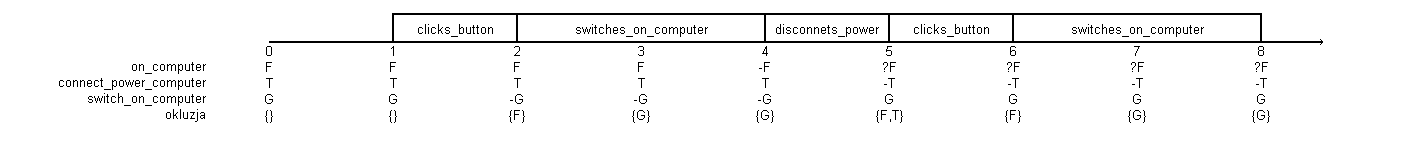
\includegraphics[width=1\textwidth]{Example5}
\end{center}



%</tag>
\end{document}
